\documentclass[11pt]{exam}
\usepackage[margin=1in]{geometry}
\usepackage{amsfonts, amsmath, amssymb, amsthm}
\usepackage{mathtools}
\usepackage{enumerate}
\usepackage{listings}
\usepackage{colortbl}
\usepackage{float}
\usepackage{algorithm}
\usepackage{algorithmic}
\usepackage[colorlinks,linkcolor=blue]{hyperref}

% in order to compile this file you need to get 'header.tex' from
% Canvas and change the line below to the appropriate file path
%%% theorems

\theoremstyle{plain}            % following are "theorem" style
\newtheorem{theorem}{Theorem}[section]
\newtheorem{lemma}[theorem]{Lemma}
\newtheorem{corollary}[theorem]{Corollary}
\newtheorem{proposition}[theorem]{Proposition}
\newtheorem{claim}[theorem]{Claim}
\newtheorem{fact}[theorem]{Fact}
\newtheorem{openproblem}[theorem]{Open Problem}

\theoremstyle{definition}       % following are def style
\newtheorem{definition}[theorem]{Definition}
\newtheorem{conjecture}[theorem]{Conjecture}
\newtheorem{example}[theorem]{Example}
\newtheorem{protocol}[theorem]{Protocol}
\newtheorem{exercise}[theorem]{Exercise}

\theoremstyle{remark}           % following are remark style
\newtheorem{remark}[theorem]{Remark}
\newtheorem{note}[theorem]{Note}
%\newtheorem*{solution}{Solution}

%%% special sets
\newcommand{\bit}{\ensuremath{\{0,1\}}}
\newcommand{\bitt}{\ensuremath{\{-1,1\}}}
\newcommand{\ball}{\ensuremath{\mathcal{B}}}
\newcommand{\sph}{\ensuremath{\mathbb{S}}}
\newcommand{\odisc}[2]{\ensuremath{D(#1, #2)}}
\newcommand{\cdisc}[2]{\ensuremath{\bar{D}(#1, #2)}}
\newcommand{\emp}{\varnothing}

% constants
\newcommand{\E}{\ensuremath{\mathrm{e}}}
\newcommand{\I}{\ensuremath{\mathrm{i}}}
\newcommand{\Id}{\ensuremath{\mathrm{I}}}
\newcommand{\paulix}{\ensuremath{\mathrm{X}}}
\newcommand{\pauliy}{\ensuremath{\mathrm{Y}}}
\newcommand{\pauliz}{\ensuremath{\mathrm{Z}}}

% font for general-purpose algorithms
\newcommand{\algo}[1]{\ensuremath{\mathsf{#1}}}
% font for general-purpose computational problems
\newcommand{\problem}[1]{\ensuremath{\mathsf{#1}}}
% font for complexity classes
\newcommand{\class}[1]{\ensuremath{\mathsf{#1}}}

% asymptotics
\DeclareMathOperator{\poly}{poly}
\DeclareMathOperator{\polylog}{polylog}
\DeclareMathOperator{\negl}{negl}
\DeclareMathOperator{\bigO}{O}
\DeclareMathOperator{\litO}{o}
\DeclareMathOperator{\Otil}{\tilde{O}}
\DeclareMathOperator{\Ostar}{O^*}

%%% "LEFT-RIGHT" PAIRS OF SYMBOLS

% inner product
\DeclarePairedDelimiter\inner{\langle}{\rangle}
% absolute value
\DeclarePairedDelimiter\abs{\lvert}{\rvert}
% a set
\DeclarePairedDelimiter\set{\{}{\}}
% parens
\DeclarePairedDelimiter\parens{(}{)}
% tuple, alias for parens
\DeclarePairedDelimiter\tuple{(}{)}
% square brackets
\DeclarePairedDelimiter\bracks{[}{]}
% rounding off
\DeclarePairedDelimiter\round{\lfloor}{\rceil}
% floor function
\DeclarePairedDelimiter\floor{\lfloor}{\rfloor}
% ceiling function
\DeclarePairedDelimiter\ceil{\lceil}{\rceil}
% length of some vector, element
\DeclarePairedDelimiter\length{\lVert}{\rVert}
% "lifting" of a residue class
\DeclarePairedDelimiter\lift{\llbracket}{\rrbracket}
\DeclarePairedDelimiter\len{\lvert}{\rvert}
% bra-kets
\DeclarePairedDelimiter\bra{\langle}{\rvert}
\DeclarePairedDelimiter\ket{\lvert}{\rangle}
\newcommand{\braket}[2]{\ensuremath{\langle #1 \vert #2 \rangle}}
\newcommand{\ketbra}[2]{\ensuremath{\lvert #1 \rangle \langle #2 \rvert}}

%%% spacing

\newcommand{\ws}{\hspace{1pt}}
\newcommand{\wws}{\hspace{2pt}}
\newcommand{\hs}{\hspace{4pt}}
\newcommand{\hhs}{\hspace{8pt}}
\newcommand{\hhhs}{\hspace{12pt}}

%%% LISTS

\newcommand{\oneto}{1, \ldots,}
\newcommand{\onetop}{1 \cdots,}
\newcommand{\zeroto}{0, \ldots,}
\newcommand{\zerotop}{0 \cdots,}
\newcommand{\perm}[1]{\mathbf{(#1)}}
\newcommand{\permv}[1]{(#1)}
\newcommand{\varind}[2]{#1_1, \ldots, #1_#2}
\newcommand{\varindz}[2]{#1_0, \ldots, #1_#2}
\newcommand{\varindp}[2]{#1_1 \cdots #1_#2}
\newcommand{\varindpz}[2]{#1_0 \cdots #1_#2}
\newcommand{\seq}[2]{(#1_#2)_{#2=1}^\infty}
\newcommand{\seqz}[2]{(#1_#2)_{#2=0}^\infty}

%%% MATH OPERATORS

%\DeclareMathOperator{\pr}{\mathbf{P}}
%\DeclareMathOperator{\ex}{\mathbf{E}}
\DeclareMathOperator{\pr}{P}
\DeclareMathOperator{\ex}{E}
\DeclareMathOperator{\Span}{Span}
\DeclareMathOperator{\tr}{Tr}
\DeclareMathOperator{\supp}{Supp}
\DeclareMathOperator{\im}{Im}
\DeclareMathOperator{\var}{var}
\DeclareMathOperator{\vol}{vol}
\DeclareMathOperator{\sign}{sign}
\DeclareMathOperator{\dkl}{D_{KL}}
\DeclareMathOperator{\entr}{H}
\DeclareMathOperator{\fid}{F}
\DeclareMathOperator{\dist}{D}
\DeclareMathOperator{\ad}{ad}

% hats

\newcommand{\fhat}{\ensuremath{\hat{f}}}
\newcommand{\phat}{\ensuremath{\hat{p}}}
\newcommand{\that}{\ensuremath{\hat{t}}}

%%% BLACKBOARD SYMBOLS

% \newcommand{\C}{\ensuremath{\mathbb{C}}}
\newcommand{\D}{\ensuremath{\mathbb{D}}}
\newcommand{\F}{\ensuremath{\mathbb{F}}}
% \newcommand{\G}{\ensuremath{\mathbb{G}}}
\newcommand{\J}{\ensuremath{\mathbb{J}}}
\newcommand{\N}{\ensuremath{\mathbb{N}}}
\newcommand{\Q}{\ensuremath{\mathbb{Q}}}
\newcommand{\R}{\ensuremath{\mathbb{R}}}
\newcommand{\T}{\ensuremath{\mathbb{T}}}
\newcommand{\Z}{\ensuremath{\mathbb{Z}}}
\newcommand{\QR}{\ensuremath{\mathbb{QR}}}

% sets in calligraphic type

\newcommand{\calD}{\ensuremath{\mathcal{D}}}
\newcommand{\calF}{\ensuremath{\mathcal{F}}}
\newcommand{\calG}{\ensuremath{\mathcal{G}}}
\newcommand{\calH}{\ensuremath{\mathcal{H}}}
\newcommand{\calI}{\ensuremath{\mathcal{I}}}
\newcommand{\calL}{\ensuremath{\mathcal{L}}}
\newcommand{\calN}{\ensuremath{\mathcal{N}}}
\newcommand{\calP}{\ensuremath{\mathcal{P}}}
\newcommand{\calS}{\ensuremath{\mathcal{S}}}
\newcommand{\calX}{\ensuremath{\mathcal{X}}}
\newcommand{\calY}{\ensuremath{\mathcal{Y}}}

% matrices and vectors

\newcommand{\matA}{\ensuremath{\mathbf{A}}}
\newcommand{\matB}{\ensuremath{\mathbf{B}}}
\newcommand{\matC}{\ensuremath{\mathbf{C}}}
\newcommand{\matD}{\ensuremath{\mathbf{D}}}
\newcommand{\matE}{\ensuremath{\mathbf{E}}}
\newcommand{\matF}{\ensuremath{\mathbf{F}}}
\newcommand{\matG}{\ensuremath{\mathbf{G}}}
\newcommand{\matH}{\ensuremath{\mathbf{H}}}
\newcommand{\matI}{\ensuremath{\mathbf{I}}}
\newcommand{\matJ}{\ensuremath{\mathbf{J}}}
\newcommand{\matK}{\ensuremath{\mathbf{K}}}
\newcommand{\matL}{\ensuremath{\mathbf{L}}}
\newcommand{\matM}{\ensuremath{\mathbf{M}}}
\newcommand{\matN}{\ensuremath{\mathbf{N}}}
\newcommand{\matO}{\ensuremath{\mathbf{O}}}
\newcommand{\matP}{\ensuremath{\mathbf{P}}}
\newcommand{\matQ}{\ensuremath{\mathbf{Q}}}
\newcommand{\matR}{\ensuremath{\mathbf{R}}}
\newcommand{\matS}{\ensuremath{\mathbf{S}}}
\newcommand{\matT}{\ensuremath{\mathbf{T}}}
\newcommand{\matU}{\ensuremath{\mathbf{U}}}
\newcommand{\matV}{\ensuremath{\mathbf{V}}}
\newcommand{\matW}{\ensuremath{\mathbf{W}}}
\newcommand{\matX}{\ensuremath{\mathbf{X}}}
\newcommand{\matY}{\ensuremath{\mathbf{Y}}}
\newcommand{\matZ}{\ensuremath{\mathbf{Z}}}
\newcommand{\matzero}{\ensuremath{\mathbf{0}}}

\newcommand{\veca}{\ensuremath{\mathbf{a}}}
\newcommand{\vecb}{\ensuremath{\mathbf{b}}}
\newcommand{\vecc}{\ensuremath{\mathbf{c}}}
\newcommand{\vecd}{\ensuremath{\mathbf{d}}}
\newcommand{\vece}{\ensuremath{\mathbf{e}}}
\newcommand{\vecf}{\ensuremath{\mathbf{f}}}
\newcommand{\vecg}{\ensuremath{\mathbf{g}}}
\newcommand{\vech}{\ensuremath{\mathbf{h}}}
\newcommand{\veck}{\ensuremath{\mathbf{k}}}
\newcommand{\vecm}{\ensuremath{\mathbf{m}}}
\newcommand{\vecp}{\ensuremath{\mathbf{p}}}
\newcommand{\vecq}{\ensuremath{\mathbf{q}}}
\newcommand{\vecr}{\ensuremath{\mathbf{r}}}
\newcommand{\vecs}{\ensuremath{\mathbf{s}}}
\newcommand{\vect}{\ensuremath{\mathbf{t}}}
\newcommand{\vecu}{\ensuremath{\mathbf{u}}}
\newcommand{\vecv}{\ensuremath{\mathbf{v}}}
\newcommand{\vecw}{\ensuremath{\mathbf{w}}}
\newcommand{\vecx}{\ensuremath{\mathbf{x}}}
\newcommand{\vecy}{\ensuremath{\mathbf{y}}}
\newcommand{\vecz}{\ensuremath{\mathbf{z}}}
\newcommand{\veczero}{\ensuremath{\mathbf{0}}}
\newcommand{\vecone}{\ensuremath{\mathbf{1}}}

\newcommand{\vecell}{\ensuremath{\boldsymbol\ell}}
\newcommand{\vecalpha}{\ensuremath{\boldsymbol\alpha}}
\newcommand{\vecbeta}{\ensuremath{\boldsymbol\beta}}
\newcommand{\veceta}{\ensuremath{\boldsymbol\eta}}
\newcommand{\vecmu}{\ensuremath{\boldsymbol\mu}}
\newcommand{\vecphi}{\ensuremath{\boldsymbol\phi}}
\newcommand{\vecsigma}{\ensuremath{\boldsymbol\sigma}}
\newcommand{\vectheta}{\ensuremath{\boldsymbol\theta}}
\newcommand{\vecxi}{\ensuremath{\boldsymbol\xi}}

%%% misc

\newcommand{\ind}{\ensuremath{\mathbf{1}}}

\newcommand{\congmod}[3]{#1 \equiv #2 \textrm{ modulo } #3}

\newcommand{\dee}{\,\mathrm{d}}
\newcommand{\de}{\mathrm{d}}
\newcommand{\dx}{\,\mathrm{d} x}

\newcommand{\ol}{\overline}
\newcommand{\inv}[1]{\ensuremath{#1^{-1}}}
\newcommand{\tsp}[1]{\ensuremath{#1^{\top}}}


\newcommand{\eps}{\varepsilon}
\newcommand{\ph}{\varphi}

\newcommand{\Ra}{\Rightarrow}
\newcommand{\Lra}{\Leftrightarrow}
\newcommand{\rsqa}{\rightsquigarrow}

\newcommand{\trl}{\triangleleft}
\newcommand{\trr}{\triangleright}

\newcommand{\func}[3]{#1: #2 \to #3}
\newcommand{\dd}[1]{\frac{\mathrm{d}}{\mathrm{d}#1}}
\newcommand{\ptl}[1]{\frac{\partial}{\partial #1}}
\newcommand{\prtl}[2]{\frac{\partial #1}{\partial #2}}

\newcommand{\matrixtt}[4]{
  \begin{pmatrix*}[r]
        #1 & #2 \\
        #3 & #4
    \end{pmatrix*}
}

%%% for homework and section notes

\newcommand{\commonheader}[2]{
    \pagestyle{headandfoot}
    \setlength{\headheight}{26pt}
    \setlength{\headsep}{30pt}

    \header
        {\small{\textbf{VE281: Data Structures and Algorithms}} \\ \footnotesize{\textbf{UM-SJTU Joint Institute, FA2021}}}
        {#1}
        {#2}

    \firstpageheadrule
    \runningheadrule

    \footer
        {}
        {\thepage}
        {}
}

\newcommand{\hwheader}{
    \commonheader
        {\textbf{Homework \hwnum}}
        {\small \textbf{Due at \duedate}}
}

\newcommand{\hwslnheader}{
    \commonheader
    	{}
        {\textbf{Solutions to Homework \hwnum}}
    \printanswers
}

\newcommand{\notesheader}{
    \commonheader
        {\Large \textbf{Section Notes \sectionnum}}
    	{}
}

\newcommand{\hint}[1]{
\emph{Hint}: #1
}

% for effort questions
\let\Eitem=\relax
\def\effortE{\textbf{E}~}
\makeatletter
\def\Eitem{%
    \expandafter\let\expandafter\originallabel\csname labelenum\romannumeral\@enumdepth\endcsname
    \expandafter\def\csname labelenum\romannumeral\@enumdepth\expandafter\endcsname\expandafter{%
        \expandafter\effortE\originallabel}%
    \item
    \expandafter\let\csname labelenum\romannumeral\@enumdepth\endcsname\originallabel
}
\makeatother

\allowdisplaybreaks


\geometry{left=2.5 cm,right=2.5 cm,top=2.5 cm,bottom=2.5 cm}
%\pagestyle{fancy}
\definecolor{mygreen}{rgb}{0,0.6,0}  
\definecolor{mygray}{rgb}{0.5,0.5,0.5}
\definecolor{mymauve}{rgb}{0.58,0,0.82} 
\definecolor{background}{rgb}{0.963,0.963,0.963}

\definecolor{codegreen}{rgb}{0,0.6,0}
\definecolor{codegray}{rgb}{0.5,0.5,0.5}
\definecolor{codepurple}{rgb}{0.58,0,0.82}
\definecolor{backcolour}{rgb}{0.95,0.95,0.92}

\lstdefinestyle{mystyle}{
    backgroundcolor=\color{backcolour},   
    commentstyle=\color{codegreen},
    keywordstyle=\color{magenta},
    numberstyle=\tiny\color{codegray},
    stringstyle=\color{codepurple},
    basicstyle=\ttfamily\footnotesize,
    breakatwhitespace=false,         
    breaklines=true,                 
    captionpos=b,                    
    keepspaces=true,                 
    numbers=left,                    
    numbersep=5pt,                  
    showspaces=false,                
    showstringspaces=false,
    showtabs=false,                  
    tabsize=2,
    language=c++
}

\lstset{style=mystyle}
\newcommand{\hwnum}{5}
\newcommand{\duedate}{11:59pm, December 8th}

%\notesheader
\hwheader   % header for homework
%\hwslnheader   % header for homework solutions

% Comment the following line in order to hide solutions.
% Uncomment the line to show solutions written inside of
% LaTeX solution environments like:
%   \begin{solution}
%     My solution.
%   \end{solution}.
\printanswers

\begin{document}
\setlength{\parindent}{0pt}
\section*{Before you start:}

\subsection*{Homework Files}
You can download the starter files for coding as well as this \textit{tex} file (you only need to modify \textit{homework\hwnum.tex}) on canvas and do your homework with latex. Or you can scan your handwriting, convert to pdf file, and upload it to canvas before the due date. If you choose to write down your answers by hand, you can directly download the pdf file on canvas which provides more blank space for solution box.

\subsection*{Submission Form}
For homework \hwnum, there are only one part of submission, which is a pdf file as your solution named as VE281\_HW\hwnum\_[Your Student ID]\_[Your name].pdf uploaded to canvas.

Estimated time used for this homework: \textbf{4-5 hours.}
\\\\
Great credits to 2020FA VE281 TA Group and enormous thanks to 2021SU VE281 TA Roihn!!!

\newpage
\section*{0\quad Student Info (0 point)}
Your name and student id:
\begin{solution}
% Write your answer here
\end{solution}

\section{Dynamic Programming (60 points)}
\subsection{Basic Case (12 points)}
Suppose that we have an $n*n$ matrix filled with integers. Starting from the top left corner, we advance to either the downward or rightward block for each step and finally reach the bottom right corner of the matrix. During this process, we will pass through nodes with different integers. By applying dynamic programming, we can find the path with the largest sum of the passed integers. Write out the recurrence relation.
\begin{solution}
% Write your solution here.
\end{solution}
\subsection{Do it twice? (24 points)}
Previously, we just go across the matrix for a single time. Assume that after the first travel, we set the visited integer in the matrix to be 0 and go across the matrix, back to the left corner again. How to maximize the sum of the passed integers in the whole procedure (top left -> bottom right -> top left)? In terms of this problem, William and Coned have different ideas again.
\subsubsection{Simple repeat (10 points)}
Coned thinks that since this problem is quite similar to what we have solved in 1.1, just {\color{blue}run dynamic programming twice} and add them up, and we will have the correct final result. Do you agree with him? If agree, write the recurrence relation for the second dynamic programming procedure and state whether there is a difference; if not agree, come up with a counter example and explain why it doesn't work.
\begin{solution}
% Write your solution here.
\end{solution}
\subsubsection{Double the result table (14 points)}
William thinks that the dynamic programming strategy for this problem should be {\color{blue}modified from the very beginning} in this case. He gives out the main function as shown below. However, after testing, he found out there are some problems within this piece of code. Please correct the code between line 17 to line 26.
\newpage 
\begin{lstlisting}
int main(){
    // two paths are considered simultaneously, one at (i, j), the other at (k, l)
    // integers stored in integer[n][n]
    int n;
    cin >> n;
    int dp[100][100][100][100] = {0};
    int integers[100][100] = {0};
    // read all the inputs
    for (int i = 0; i < n; i++)
        for (int j = 0; j < n; j++)
            cin >> integers[i][j];
    
    dp[0][0][0][0] = integers[0][0]; // start point
    
    // start dp
    
    /* modify code within this part */
    for (int i = 0; i < n; i++)
        for (int j = 0; j < n; j++)
            for (int k = 0; k < n; k++)
                for (int l = 0; l < n; l++)
                    dp[i][j][k][l] = max(dp[i-1][j][k-1][l], dp[i][j-1][k-1][l],
                                         dp[i-1][j][k][l-1], dp[i][j-1][k][l-1]);
                                         
                                         
    /* modify code within this part */
    
    cout << dp[n][n][n][n];
    
}
\end{lstlisting}
\subsection{How to save memory? (12 points)}
Coned takes a look at William's strategy and thinks that its memory usage is too bad. Regardless of correctness, it will have a space complexity of $O(n^4)$, which sounds horrible. Propose a modification to this dynamic programming algorithm so that the space complexity can be reduced to $O(n^3)$ and write out its recurrence relation.\\
Hint: one way to do so is to reduce the array $dp$ to be 3-dimensional. There should be 1 dimension still for $i$ and 1 dimension still for $k$.
\begin{solution}
% Write your solution here
\end{solution}
\subsection{Does optimization end here? (12 points)}
Looking at the modification proposed by Coned, William surprisingly agrees with him. After brainstorming, they find that this strategy can be further optimized in terms of space complexity. Briefly state how you can further reduce its space complexity to $O({\color{red}2}n^2)$.\\
Hint: Do we need every $dp$ value in every iteration?
\begin{solution}
% Write your solution here
\end{solution}
Notes: Actually we can further reduce its space usage from $O(2n^2)$ to $O(n^2)$ in this problem.
\newpage
\section{Self-balanced tree (40 points)}
\subsection{AVL Tree (20 points)}
\subsubsection{Rotate! (6 points)}
Give the shortest sequence of single left or right rotations, and the two nodes being rotated, to transform the tree on the left to the tree on the right. Indicate in the rightmost column if the tree \textbf{after} the rotation satisfies the balance invariant of the AVL trees and also write out the balance factor of the \textbf{root} after rotation.\\
Notice that there might be unnecessary rotations, but make sure your sequence exactly matches the provided final result. You don't need to fill in all the rows in the table.
\begin{center}
    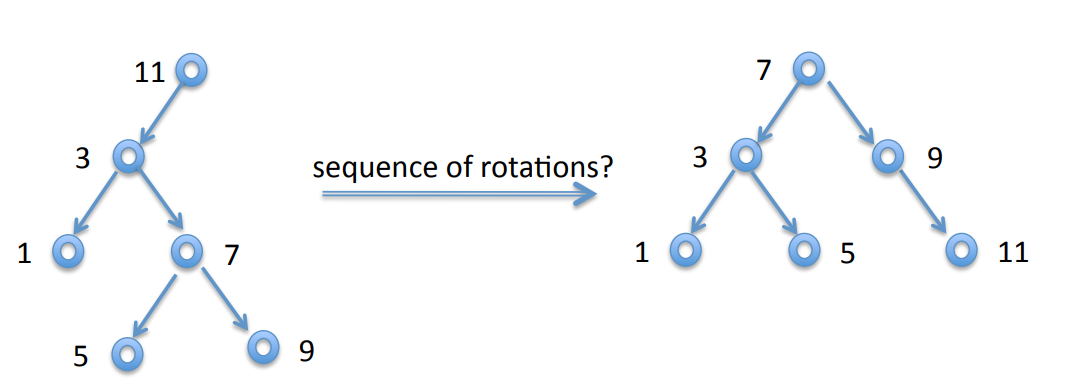
\includegraphics[scale=0.4]{AVL_rotation.png}
\end{center}
\begin{center}
    \begin{tabular}{|c|c|c|c|c|}
    \hline
    Step & Left or Right? & at nodes & balance factor & AVL? \\
    \hline
    1 & left & 3,7 & 2 & no \\
    \hline
    2 & & & & \\
    \hline
    3 & & & & \\
    \hline
    4 & & & & \\
    \hline
    5 & & & & \\
    \hline
\end{tabular}
\end{center}

\subsubsection{Simulate! (8 points)}
    Based on the balanced tree in 2.1.1, give a value whose insertion will trigger a {\color{red}left-left} rotation. If such a value does not exist, choose a non-leaf node to delete and again give such a value whose insertion will trigger a left-left rotation. Draw your final tree no matter whether a deletion takes place.\\
    Assume that when deleting a non-leaf node, we always use the largest node in the left subtree to replace the deleted node.
    \begin{solution}
    % Write the solution
    \end{solution}
\subsubsection{Code! (6 points)}
In the lecture slides, the implementation of \lstinline{Balance()} is given. In this problem, please implement \lstinline{LLRotation} as well as \lstinline{LRRotation} to make \lstinline{Balance()} work properly. Suppose that \lstinline{RRRotation} and \lstinline{RLRotation} have been implemented and we follow the definitions in the slides.
\begin{lstlisting}[language=c++]
void LLRotation(node *&n) {
    
    
    
    
    
}
void LRRotation(node *&n) {
    
    
    
    
    
}
\end{lstlisting}

\subsection{Red Black Tree (20 points)}
\subsubsection{Balance? (4 points)}
Briefly explain why red black tree is to some extent balanced.\\
Hint: what is the characteristic of a "balanced" tree?
\begin{solution}
% Write your solution here.
\end{solution}

\subsubsection{Complex? (8 points)}
Given such a red black tree:
\begin{center}
    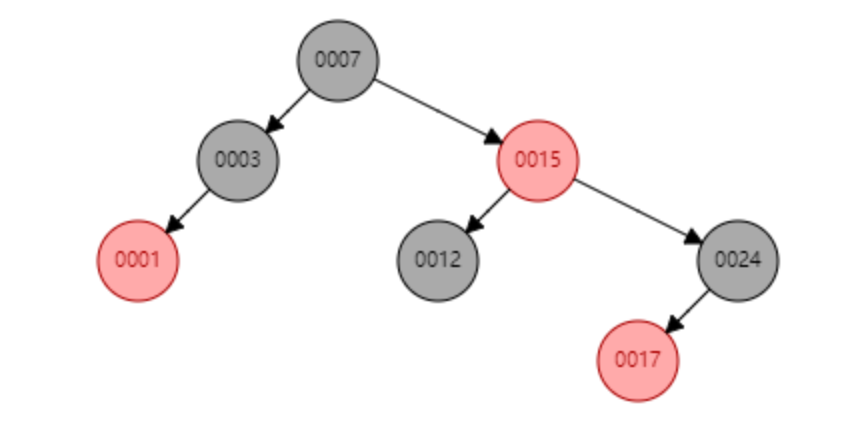
\includegraphics[scale=0.3]{rb_tree_insert.png}
\end{center}
\begin{enumerate}[1)]
    \item Show the result after inserting 20. Color the nodes clearly.
    \begin{solution}
    % Write your solution here
    \end{solution}
    \item After 1), show the result after inserting 23. Color the nodes clearly.
    \begin{solution}
    % Write your solution here
    \end{solution}
\end{enumerate}

\subsubsection{Correctness? (8 points)}
Judge whether the following red black tree is correct. If not correct, please point out which node is wrong and whether a recolor or rotation is needed (no need to draw the tree after fixing it).
\begin{enumerate}[a)]
    \item \quad\\
    \begin{center}
        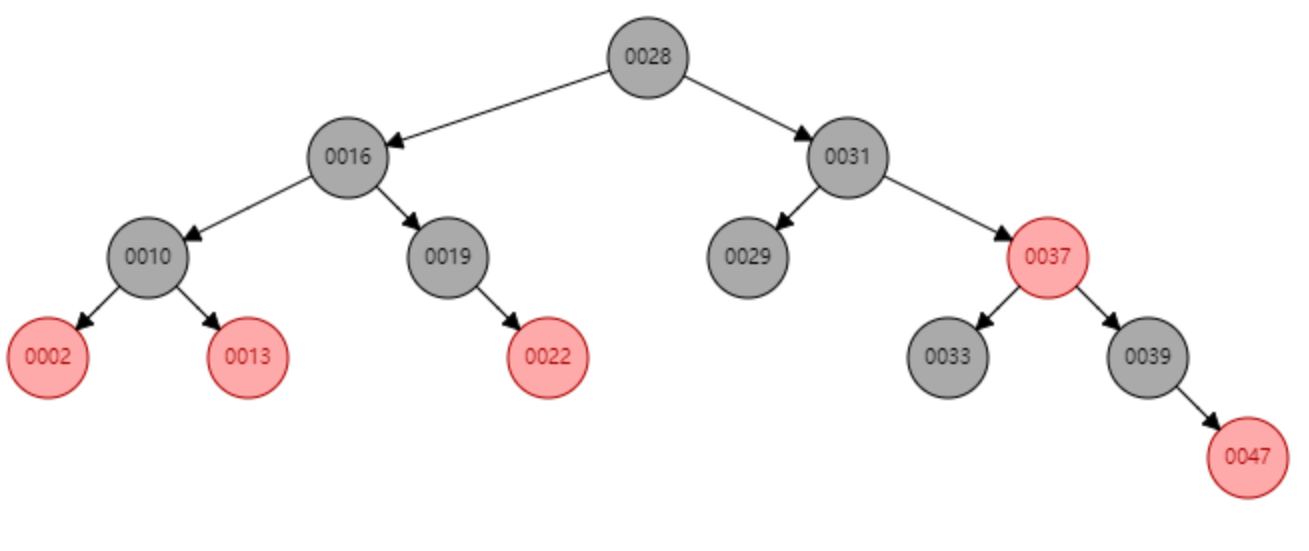
\includegraphics[scale=0.3]{rb_tree_1.png}
    \end{center}
    \begin{solution}
    % Write your solution here.
    \end{solution}
    \item \quad\\
    \begin{center}
        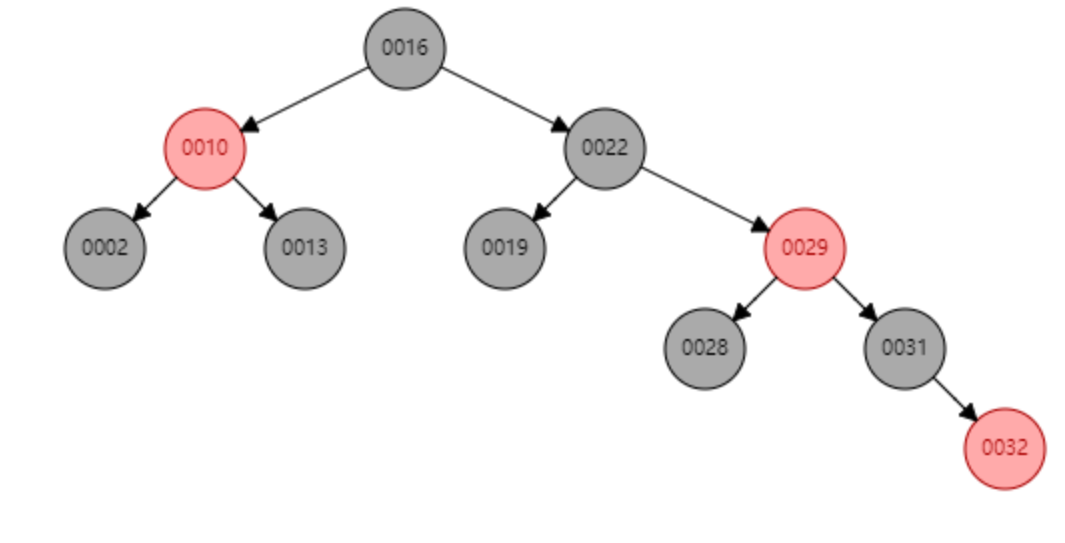
\includegraphics[scale=0.3]{rb_tree_2.png}
    \end{center}
    \begin{solution}
    % Write your solution here.
    \end{solution}
\end{enumerate}

Notes: In fact, although red black tree has a wide range of good application scenarios, its code implementation is quite complicated compared with other balanced tree such as AVL tree. It is also a reason why this assignment doesn't ask you to write related code in terms of red black tree.
\section{Your Experience}
\begin{enumerate}[1)]
    \item Please state the thing you have most positive feeling towards/like most in this course.
    \item Please state the thing you have most negative feeling towards/dislike most in this course (detailed explanation appreciated).
    \item Feel free to say any comments here!
\end{enumerate}

\section*{Reference}

Homework 6, 15-122, Carnegie Mellon University

Exam 2, 15-122, Carnegie Mellon University

\end{document}